\documentclass[standalone, version=2.0]{huangfusl-template}
\begin{document}
\begin{tabular}{cc}
    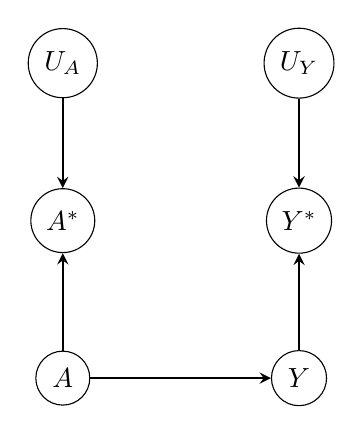
\begin{tikzpicture}
        \node[draw, circle] (As) at (0, 0) {$A^*$};
        \node[draw, circle] (Ys) at (3, 0) {$Y^*$};
        \node[draw, circle] (A) at (0, -2) {$A$};
        \node[draw, circle] (Y) at (3, -2) {$Y$};
        \node[draw, circle] (UY) at (3, 2) {$U_Y$};
        \node[draw, circle] (UA) at (0, 2) {$U_A$};

        \draw[-stealth, thick] (A) -- (Y);
        \foreach \i in {A, Y} {
            \draw[-stealth, thick] (U\i) -- (\i s);
            \draw[-stealth, thick] (\i) -- (\i s);
        }
    \end{tikzpicture} &
    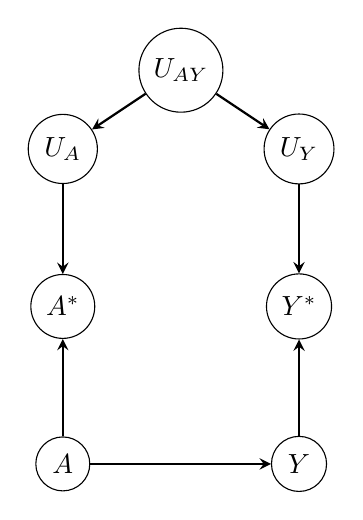
\begin{tikzpicture}
        \node[draw, circle] (UAY) at (1.5, 3) {$U_{AY}$};
        \node[draw, circle] (As) at (0, 0) {$A^*$};
        \node[draw, circle] (Ys) at (3, 0) {$Y^*$};
        \node[draw, circle] (A) at (0, -2) {$A$};
        \node[draw, circle] (Y) at (3, -2) {$Y$};
        \node[draw, circle] (UY) at (3, 2) {$U_Y$};
        \node[draw, circle] (UA) at (0, 2) {$U_A$};

        \draw[-stealth, thick] (A) -- (Y);
        \foreach \i in {A, Y} {
            \draw[-stealth, thick] (UAY) -- (U\i);
            \draw[-stealth, thick] (U\i) -- (\i s);
            \draw[-stealth, thick] (\i) -- (\i s);
        }
    \end{tikzpicture} \\
    independence & without independence
\end{tabular}
\end{document}